\documentclass{article}

\usepackage{lipsum}
\usepackage[margin=1in,includefoot]{geometry}
\usepackage{graphicx}
\usepackage{float}
\usepackage[hidelinks]{hyperref}
\usepackage{amsmath}
\usepackage{amssymb}

% Header and Footer Stuff
\usepackage{fancyhdr}
\pagestyle{fancy}
\fancyhead{}
\fancyfoot{}
\fancyfoot[R]{\thepage}
\renewcommand{\headrulewidth}{0pt}
\renewcommand{\footrulewidth}{0pt}

\begin{document}

\begin{titlepage}
	\begin{center}
	\begin{align*}
	
\includegraphics[height=1.75in]{logo.png}
	\end{align*}


	
	\line(1,0){300}\\
	[0.25in]
	\huge{\bfseries The Fourier Analysis}\\
	[2mm]
	\line(1,0){200}\\
	[1.5cm]
	\textsc{\LARGE Laboratory S1 }\\
	[0.75cm]
	\textsc{\Large 3C1 Signals and Systems}\\
	[7cm]	
	\end{center}
	
	
	
	\begin{flushright}
	\textsc{\large Alexandru Sulea\\
	D Stream\\
	\#12315152\\
	27 October 2015\\}
	\end{flushright}

\end{titlepage}
%Table of Contents Stuff%
\tableofcontents
%\listoffigures
%\addcontentsline{toc}{section}{List of Figures}
\listoftables
\addcontentsline{toc}{section}{List of Tables}


\thispagestyle{empty}
\cleardoublepage
\pagenumbering{arabic}
\setcounter{page}{1}


\section{Introduction}\label{sec:intro}
The purpose of the S1 laboratory is to examine the properties and functions Linear Time Invariant (LTI) Systems. These properties will be examined using simulation software as well as the mathematics equations associated with limited time-invariant systems.The laboratory includes the theory studied in the 3C1 Signals and Systems lectures into a practical laboratory. 
The laboratory also serves as an introduction to coding and graphing functions in Matlab. 

\section{Theory}\label{sec:theory}
\subsection{5 Signals}
Throughout this laboratory most of the signals which will be used will be sine and in some small part cos waves.\\ The sine wave is preferred over a cosine wave because it provides a clearer picture of the wave, makes it easier to determine amplitude and also, all the standard equations use the sine function. \\

\subsection{6 Linear Time Invariant System}
Limited Time Invariant Systems Theory is a way of investigating the response of a linear and time-invariant systems to an arbitrary input signal (Sine or Cosine).The trajectories of these systems are normally measured and tracked as they move through time(on the x-axis). A common example of LTI systems are electrical circuits that can be made up of resistors, capacitors, and inductors.\\


\subsection{6.1 Gain and Phase as a function of frequency}
The gain of a system is the output amplitude divided by the input amplitude , in this way we can observe how much the system has diverged from the original signal. 

The phase of a system can be measured in either seconds or by converting those seconds into radians. The phase lag is usually how faster or slower a system has changed from the original signal and the difference in time between the input and output signal. 

\pagebreak
\section{Results}\label{sec:result}
\subsection{5.1 The Sine Wave: a deterministic signal}
Q1. Using Matlab, generate the deterministic signal $$x1=3sin5t$$ and plot it over the range t=0:6 seconds. This is a sine wave.Label the x-axis as Seconds and the y-axis as Volts. Let us assume this signal is the measurement of some voltage from some AC power supply as it varies with time. Thus the plot you have made is the plot which you would see if you hooked up an Oscilloscope to the terminals of the power supply to measure Voltage.\\
Ans1.\\

\begin{align*}
\centering
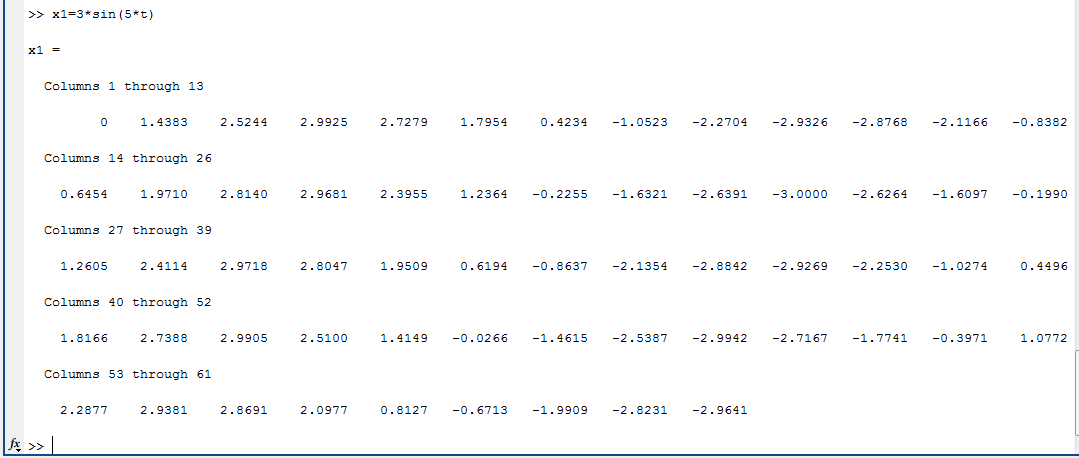
\includegraphics[height=1.75in]{S1P12.PNG}
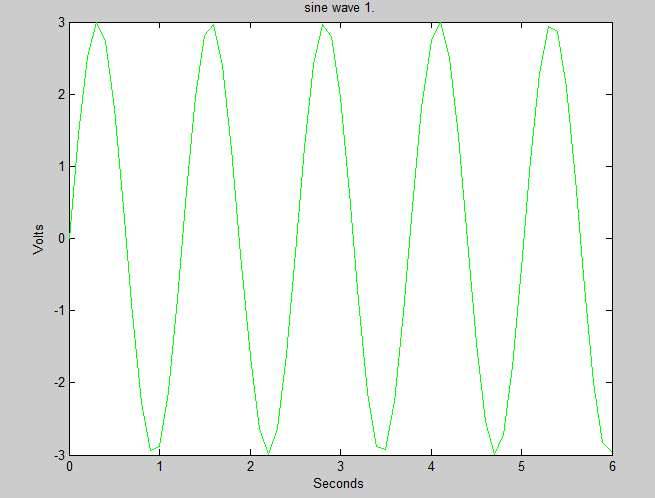
\includegraphics[height=1.75in]{S1P13.PNG}
\end{align*}\\

Q2. What is the maximum and minimum value of the sinusoid (in Volts), the frequency of the sinusoid in Hertz and the period of the wave in seconds?\\
Ans2.\\
\begin{align*}
\centering
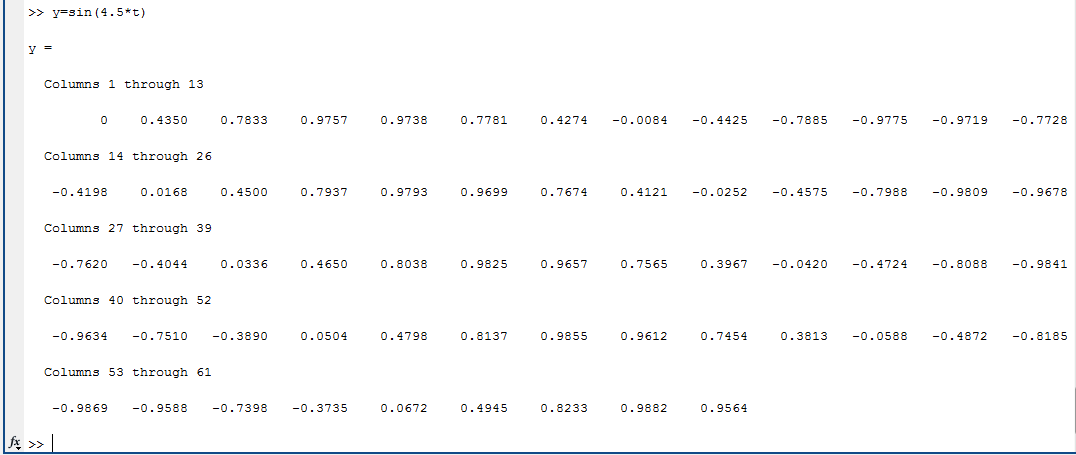
\includegraphics[height=1.75in]{S1P14.PNG}
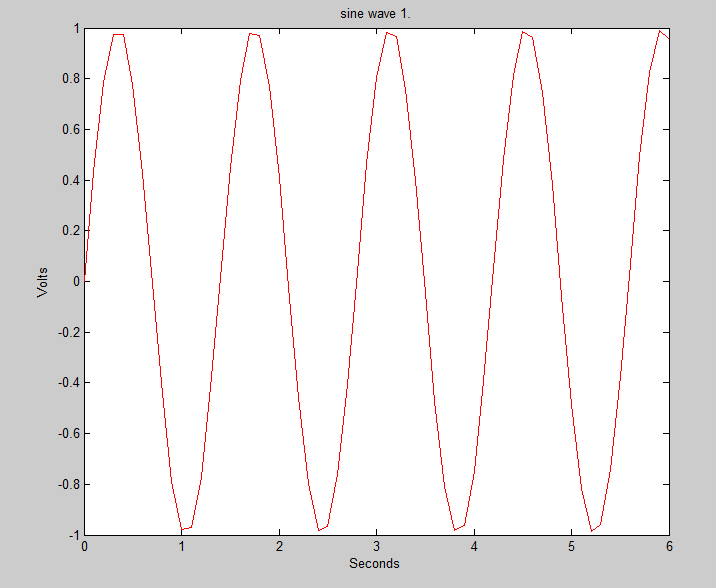
\includegraphics[height=1.75in]{S1P16.PNG}
\end{align*}\\
As can be seen from the graphs, the voltage oscillates between -1V and 1V. The period of the wave is 1.5 seconds and using these values we are able to determine that the frequency of the wave is 0.75Hz

\begin{align*}
\centering
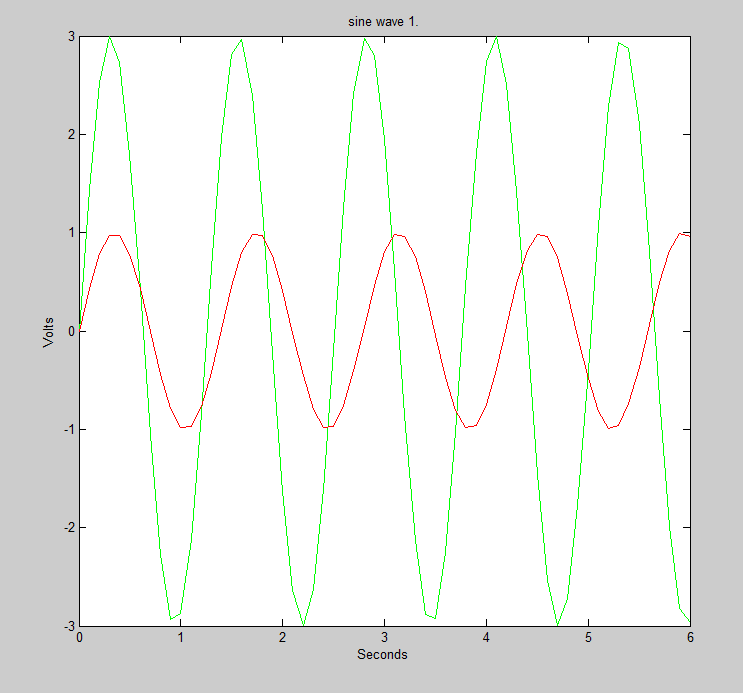
\includegraphics[height=1.75in]{S1P17.PNG}
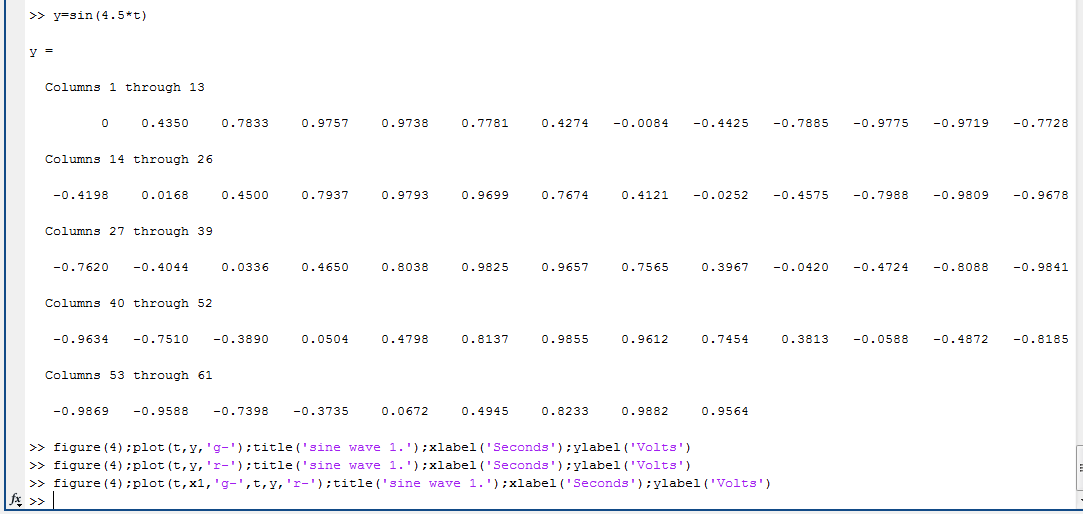
\includegraphics[height=1.75in]{S1P18.PNG}
\end{align*}\\
\begin{align*}
\centering
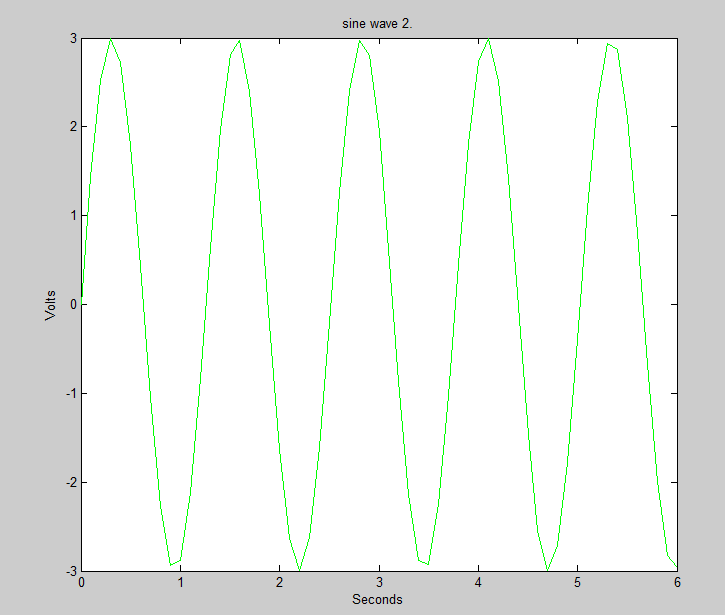
\includegraphics[height=1.75in]{S1P21.PNG}
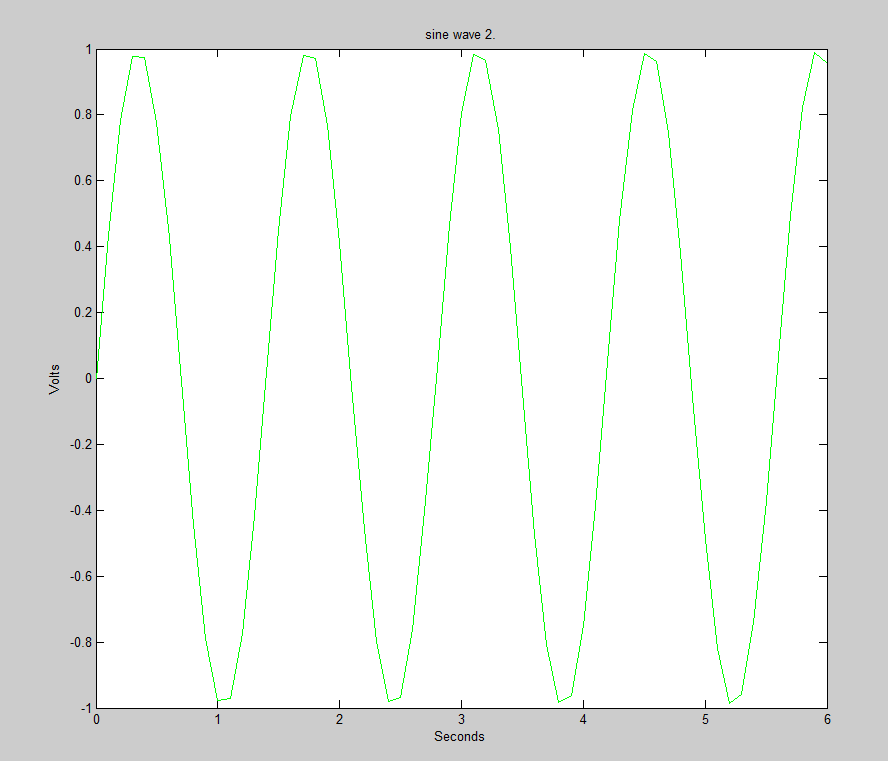
\includegraphics[height=1.75in]{S1P22.PNG}
\end{align*}\\

Q3.Use Matlab to plot the graph of x2=Asin($\omega$1(t)+$\emptyset$)
with $\omega$1=5, $\emptyset$=-3, A=3 (green color), label the axes as previously and show x1 (in red) on the same plot. Two lines should now be plotted on the graph. Include the figure in your write up.\\
What is the frequency of x2 in Hertz? What is the difference between the signals x2 and x1? Is there a phase lag?Is this a delay or an advance?\\
Ans3.\\

The frequency of x2 in Hertz is 0.75Hz. The difference between X2 and X1 is one of phase lag, both waves are sine waves and have the same amplitude yet due to the phase lag they are almost the inverse of one another. The delay is of $180^{0}$ or 0.6 seconds.

\begin{align*}
\centering
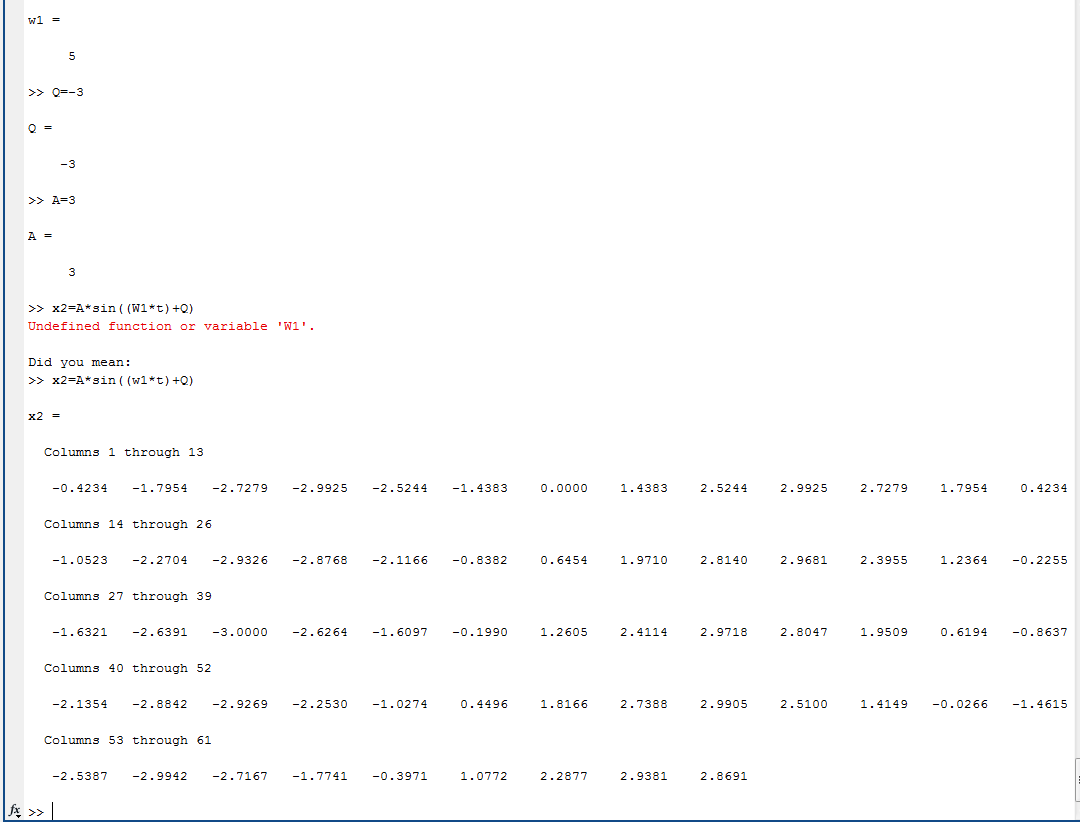
\includegraphics[height=1.75in]{S1P19.PNG}
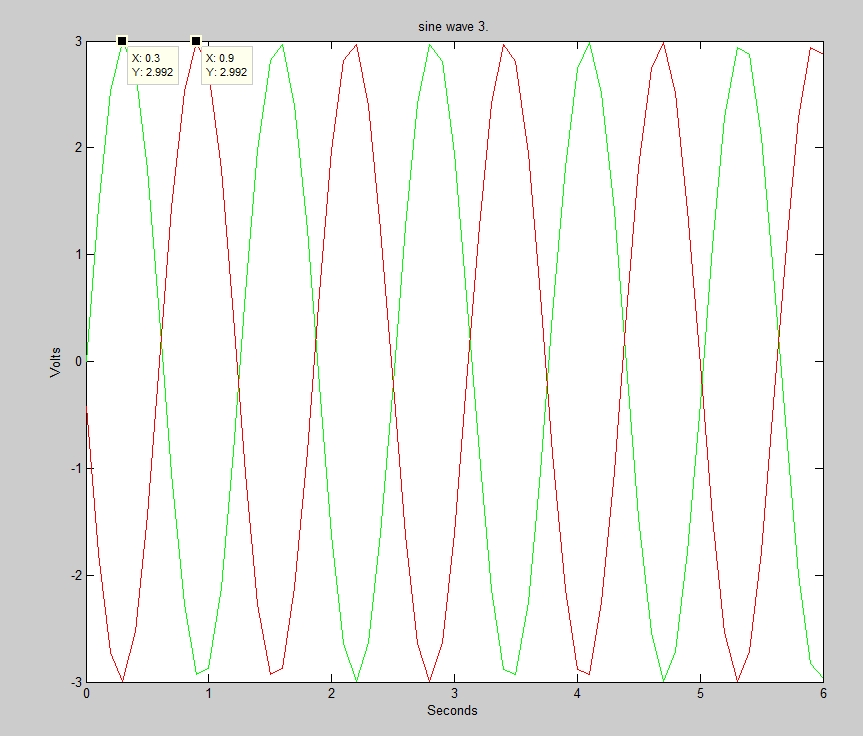
\includegraphics[height=1.75in]{S1P24.PNG}
\end{align*}\\


Q4. By how much is x2 delayed (in seconds) with respect to x1? Clearly indicate which points you used to calculate the data. How does this value relate to the constant offset term, w in the argument for the sin function in x2? Show exactly how w can be used to calculate the phase lag in seconds.\\
Ans4.\\
X2 in this instance is delayed by 0.6 seconds, as can be seen from the graph below, the top most points of each wave were used.

\begin{align*}
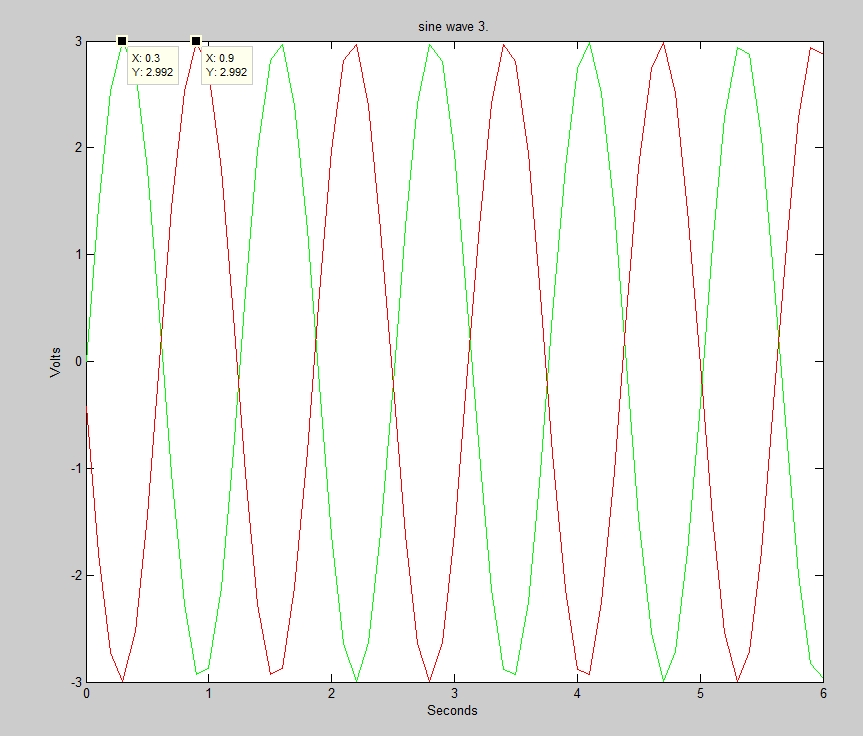
\includegraphics[height=1.75in]{S1P24.PNG}
\end{align*}\\
Q5. Use Matlab to plot the graph of x3=Asin($\omega$t+$\emptyset$) with $\omega$1=5, $\emptyset$=-3+2$\pi$, A=3. Plot the function in figure 3 superimposed on the graph for x1(as in previous instructions). By how much is x3 delayed (in seconds) with respect to x1? Use measurement from the displayed graph only. How does this value relate to the constant offset term in the argument for the sin function of x3? Explain any difference or similarity with x2 in terms of the properties of the sine function.\\
Ans5.\\

\begin{align*}
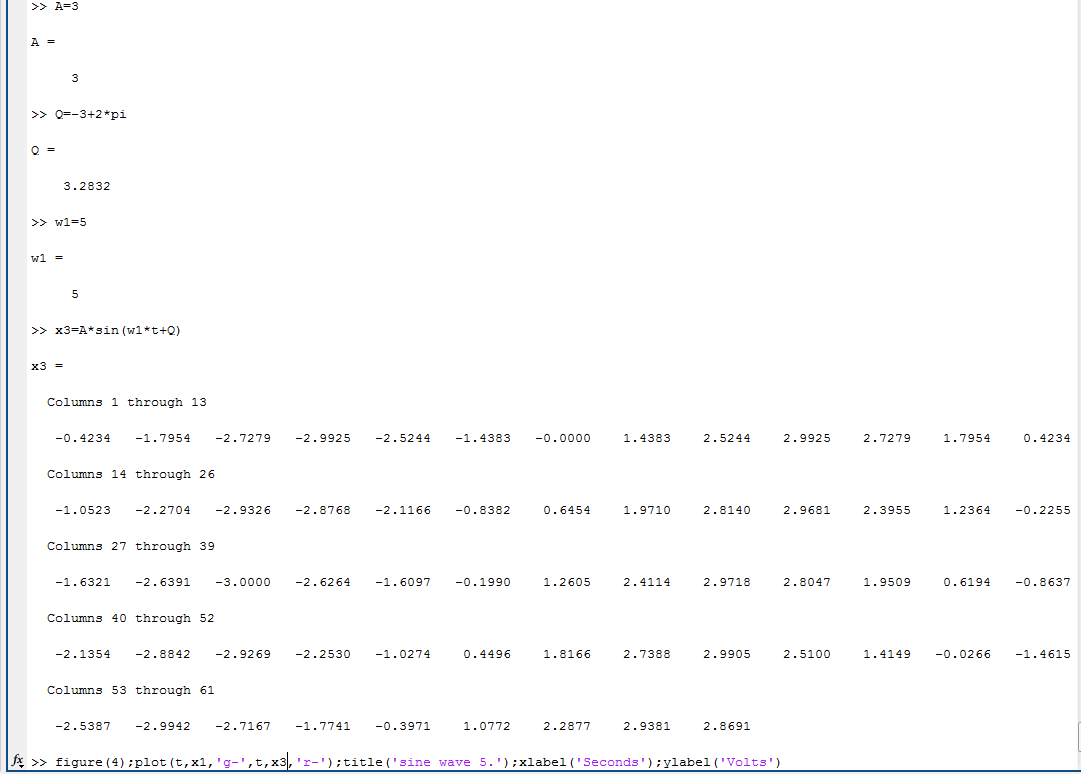
\includegraphics[height=1.75in]{S1P26.PNG}
\end{align*}\\
\begin{align*}
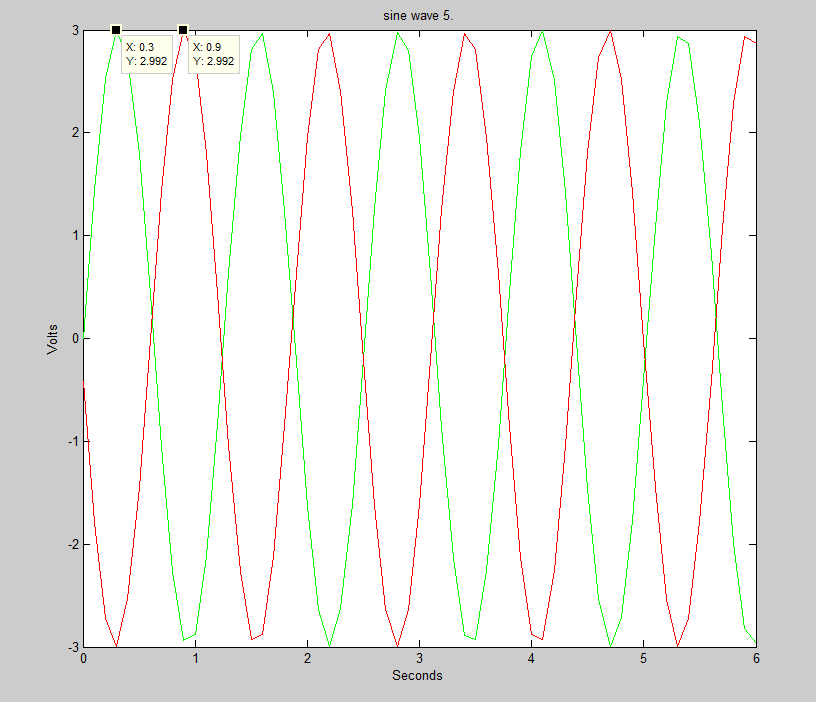
\includegraphics[height=1.75in]{S1P27.PNG}
\end{align*}\\

\subsection{6 Linear Time Invariant System}
Q1.Examine the input and output signals corresponding to the Default settings of LAB1. The input signal is a sine wave. What is the output signal?\\
\\
Ans1.

\begin{align*}
\centering
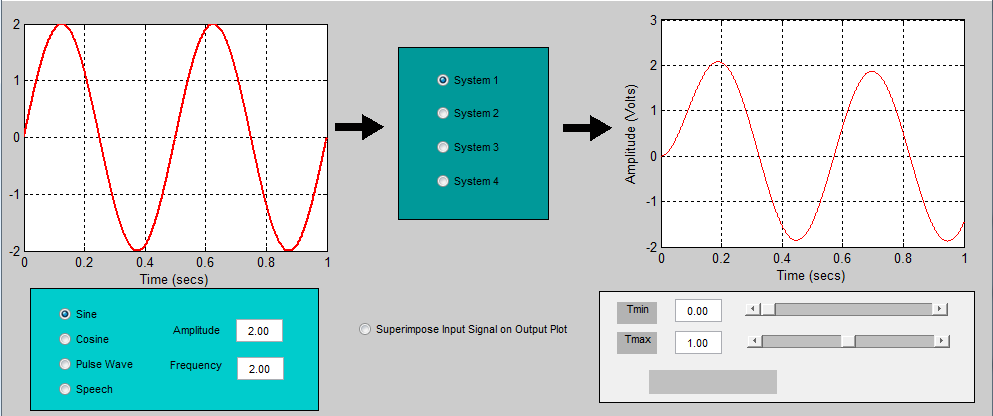
\includegraphics[height=1.75in]{S1P28.PNG}
\end{align*}
By observing the given display, output signal also seems to be a sine wave though slightly different from the original as its phase is not the same as that of the input.\\
\begin{align*}
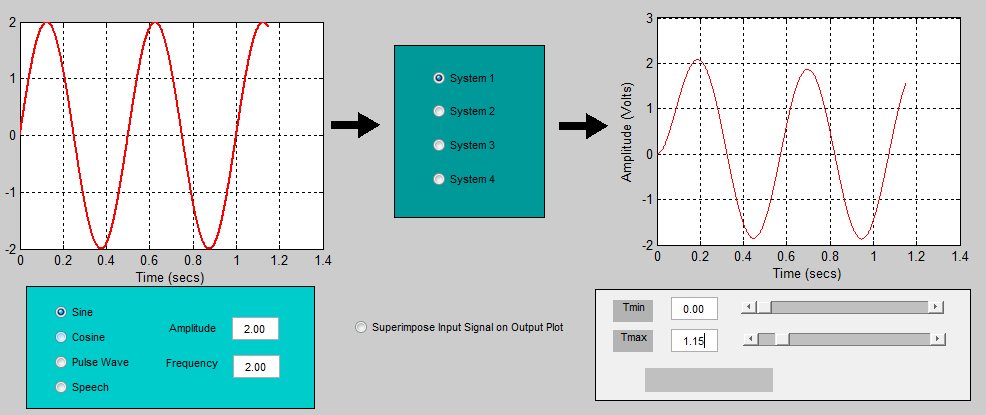
\includegraphics[height=1.75in]{S1P29.PNG}
\end{align*}

Q2.What is the difference between the input and output signals using system 1? What is the same?\\
\\
Ans2. Both the output and input signals are Sine waves. Both signals seem to have similar Amplitude. Although the signals are similar they are not identical as there is a clear and visible phase lag between input and output. The amplitude of the output is also slightly higher than that of the input.

\begin{align*}
\centering
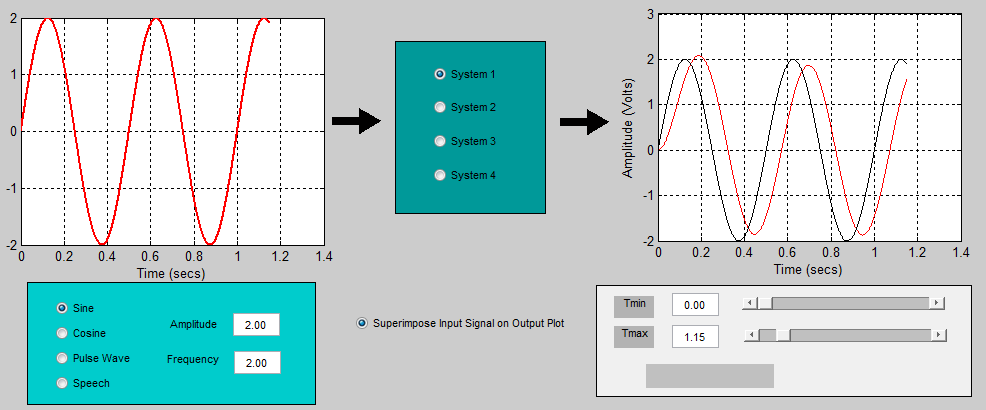
\includegraphics[height=1.75in]{S1P30.PNG}
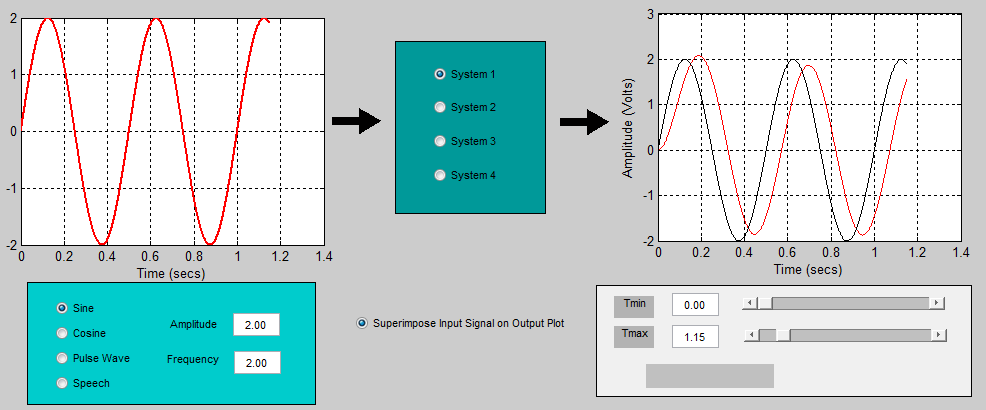
\includegraphics[height=1.75in]{S1P30.PNG}
\end{align*}

Q3.Increase the amplitude of the input signal by factor of 2. What is the corresponding increase in the amplitude of the output signal, after initial transients have decayed? How long does the system take to settle into steady state response?\\
\\
Ans3. Although not visible in the figure given, the system took 2.5 seconds to settle into a steady state response.

\begin{align*}
\centering
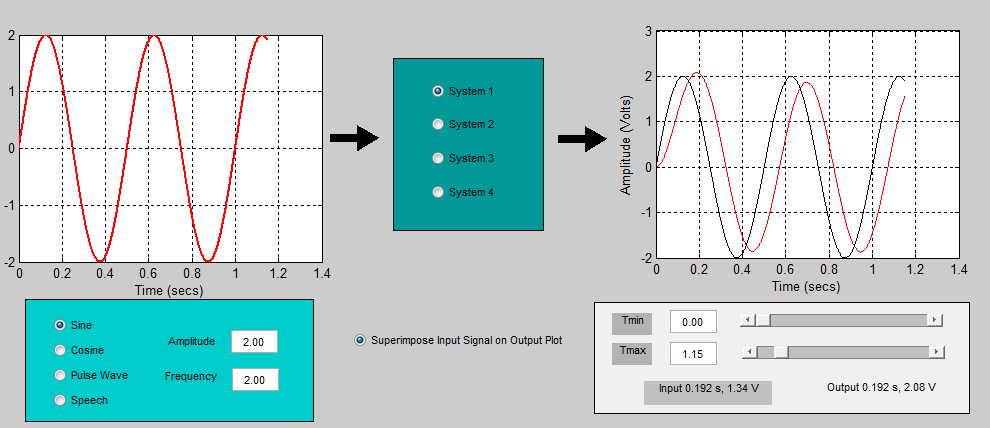
\includegraphics[height=1.75in]{S1P31.PNG}
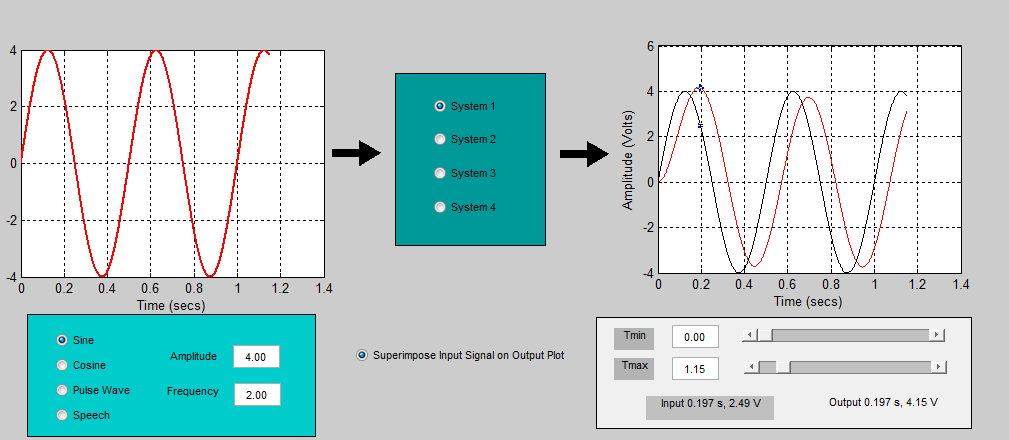
\includegraphics[height=1.75in]{S1P32.PNG}
\end{align*}

Q4. For input amplitudes of 0.5, 1.0, 1.5, 2.0, 2.5 measure the corresponding output amplitudes in the output signal and plot a graph of i/p amplitude vs. output. Label your axes carefully and include the plot in your write up.\\
\\
Ans4.\\

\begin{table}[H]
\centering
\caption{6. Q4}
\label{my-label}
\begin{tabular}{|c|c|c|c|c|c|}
\hline
       & \multicolumn{5}{c|}{Amplitude}      \\ \hline
Input  & 0.5  & 1.0   & 1.5  & 2.0   & 2.5   \\ \hline
Output & 0.52 & 1.033 & 1.56 & 2.081 & 2.601 \\ \hline
\end{tabular}
\end{table}

\begin{align*}
\centering
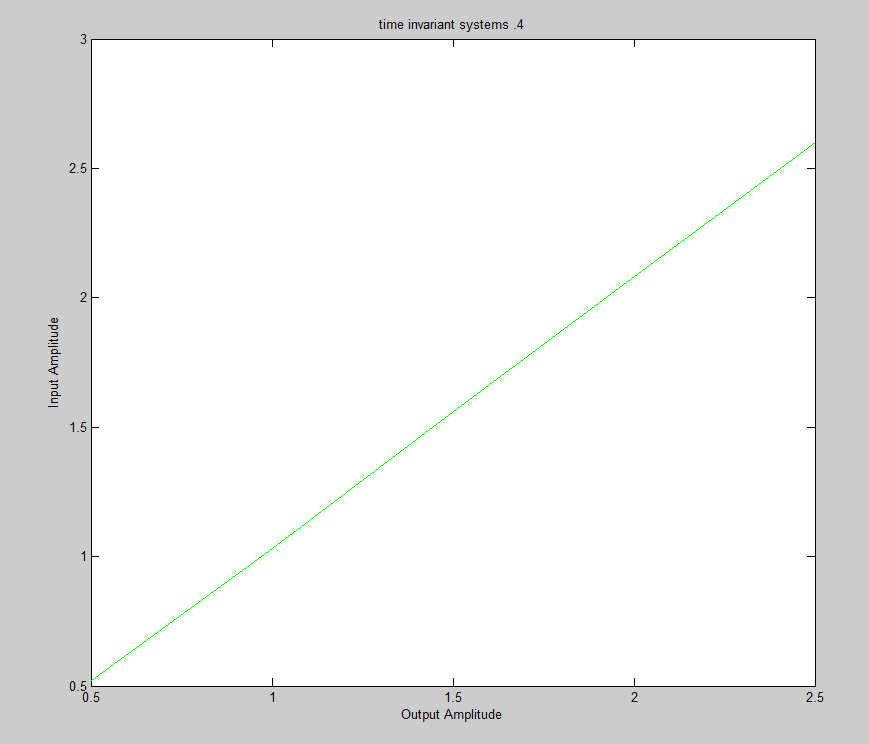
\includegraphics[height=1.75in]{S1P33.PNG}
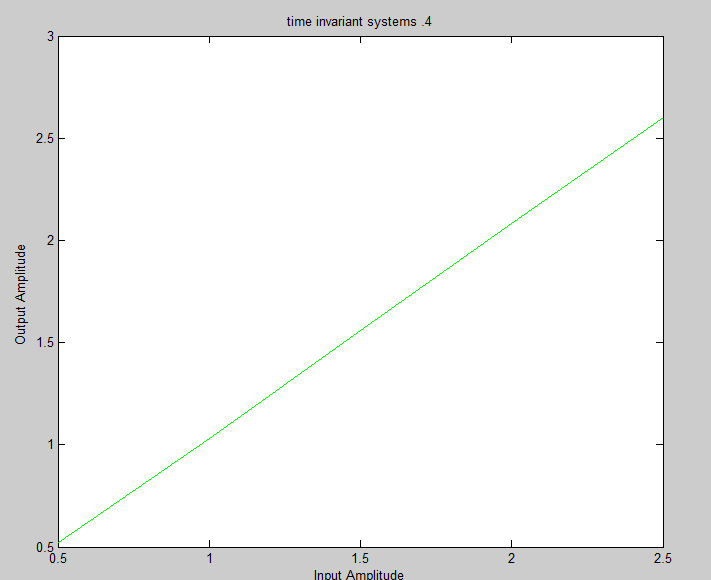
\includegraphics[height=1.75in]{S1P34.PNG}
\end{align*}


Q5. Switch the input signal to the Pulse Wave and set its frequency to 0.8Hz. and repeat the above experiment. Take the output amplitude to be the maximum value of the output pulse after initial transients have decayed.\\
\\
Ans5.
\begin{table}[H]
\centering
\caption{6. Q5.}
\label{tab: 6}
\begin{tabular}{|c|c|c|c|c|c|}
\hline
       & \multicolumn{5}{c|}{Amplitude}      \\ \hline
Input  & 0.5  & 1.0   & 1.5  & 2.0   & 2.5   \\ \hline
Output & 0.7485 & 1.497 & 2.246 & 2.994 & 3.743 \\ \hline
\end{tabular}
\end{table}

\begin{align*}
\centering
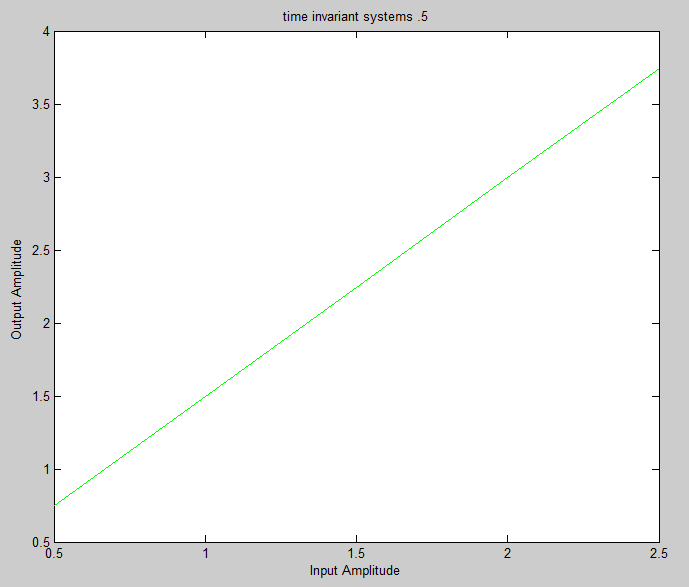
\includegraphics[height=1.75in]{S1P35.PNG}
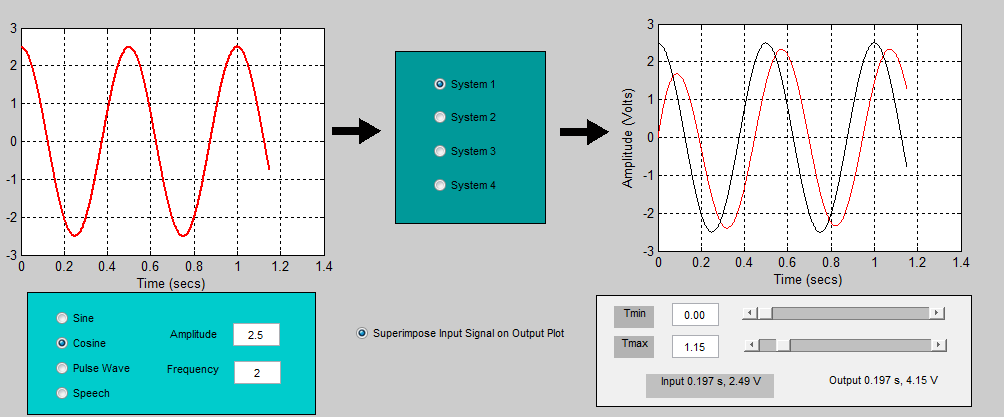
\includegraphics[height=1.75in]{S1P36.PNG}
\end{align*}

Q6. Select the Cosine as the input signal and set the frequency to 2Hz. What is the difference between the input and output signal using system 1? What is the same?\\
\\
Ans6. The similarities between the two signals are again that both signals are Sine waves which appear to be on the same frequency. 
The difference this time is that while the input signal is at a constant Amplitude the output signal starts off with a reduced amplitude and exponentially increases to match the Amplitude of the input. There is also a noticible phase lag between the two systems.\\

\begin{align*}
\centering
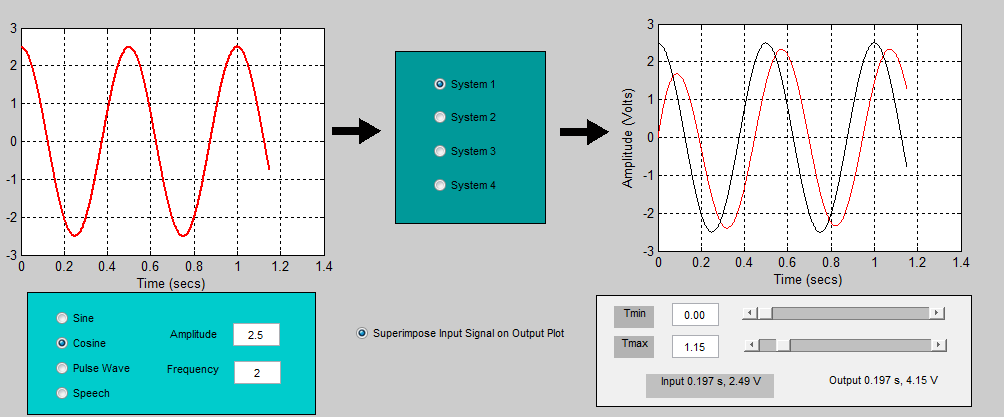
\includegraphics[height=1.75in]{S1P36.PNG}
\end{align*}
\begin{align*}
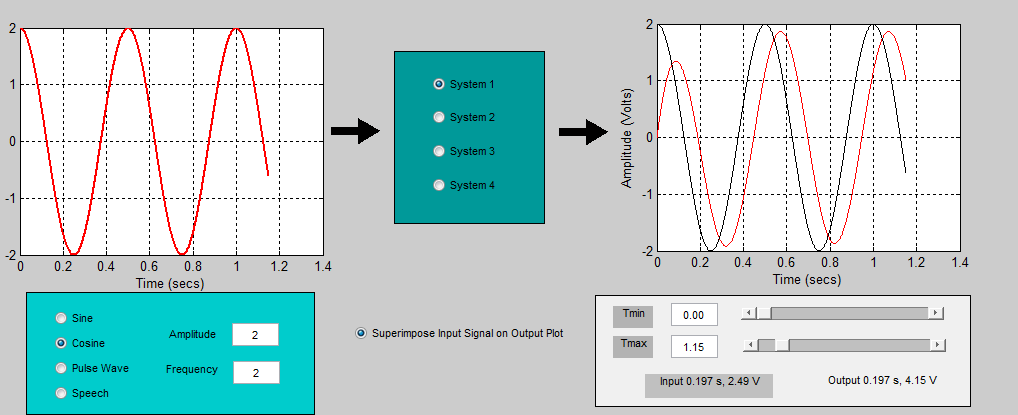
\includegraphics[height=1.75in]{S1P37.PNG}
\end{align*}\\
\begin{align*}
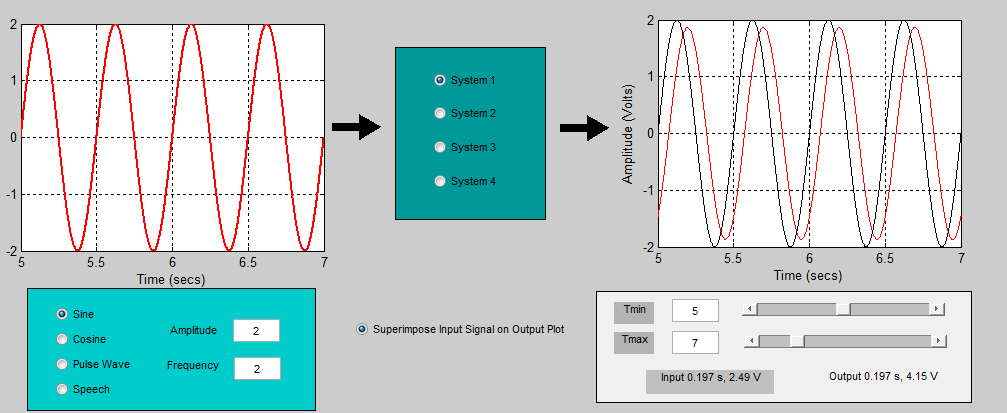
\includegraphics[height=1.75in]{S1P38.PNG}
\end{align*}


7. For both the Sine and Cosine input signals with system 1, write below matemathical expressions for the input and output signals using LAB1 to help you make measurements.\\
This final set of experiments has shown another important property of Linear systems. Complex exponential functions are eigenfunctions of Linear systems, in that they pass through a linear system without any change in shape i.e. the output signal has the same frequency as the input although changed in phase and amplitude.\\
\\
Ans7. 
$$ \int_{-\infty}^{\infty} \vert h(t) \vert dt < \infty $$
$$ \vert x(t) \vert dt \leqslant M  \quad for \quad all \quad t$$ 
$$ \vert y(t) \vert dt =  \vert \int_{-\infty}^{\infty} h(\tau) x(t-\tau) d\tau \vert$$
$$ \vert y(t) \vert dt \leqslant \int_{-\infty}^{\infty} \vert h(\tau) \vert \vert x(t-\tau) \vert d\tau$$
$$ \vert y(t) \vert dt \leqslant M \int_{-\infty}^{\infty} \vert h(\tau) \vert  d\tau < \infty \quad for \quad all \quad t$$

8. Using what you now know about LTI systems, classify Systems 2,3,4 as LTI or non-LTI.Remember to check input amplitudes covering a wide range (e.g. 1to6).\\
Ans8. Using the observed and calculated results below in the graphs, System 2 and system 4 are LTI because the input signal and output signal can be superimposed, although there is some phase lag discrepancy.
System 4 does not meet the requirements of LTI systems, the system cannot be superimposed thus it is non-LTI. \\ 

\begin{align*}
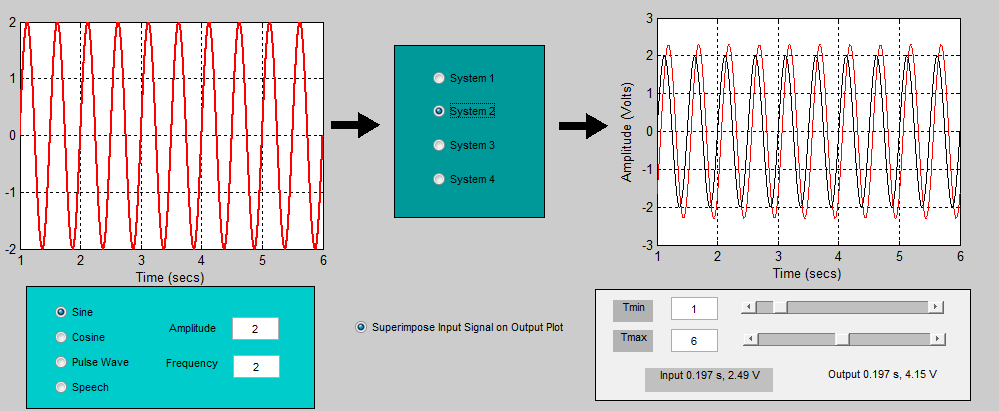
\includegraphics[height=1.75in]{S1P40.PNG}
\end{align*}\\
\begin{align*}
\centering
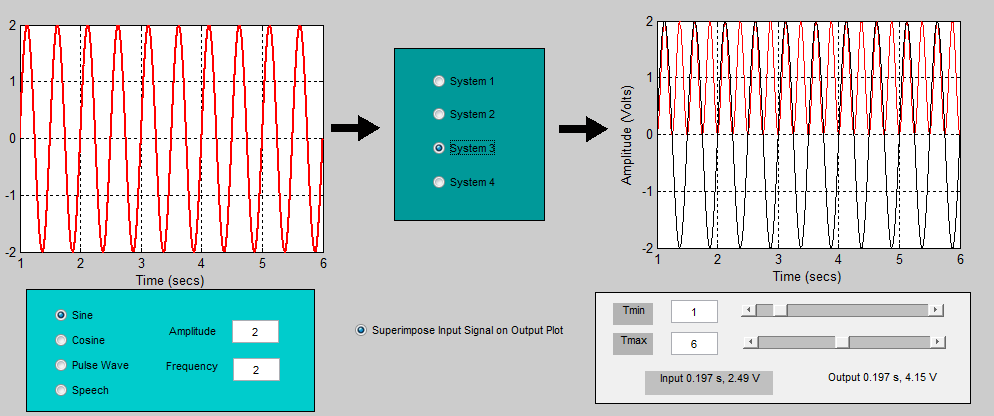
\includegraphics[height=1.75in]{S1P41.PNG}
\end{align*}\\
\begin{align*}
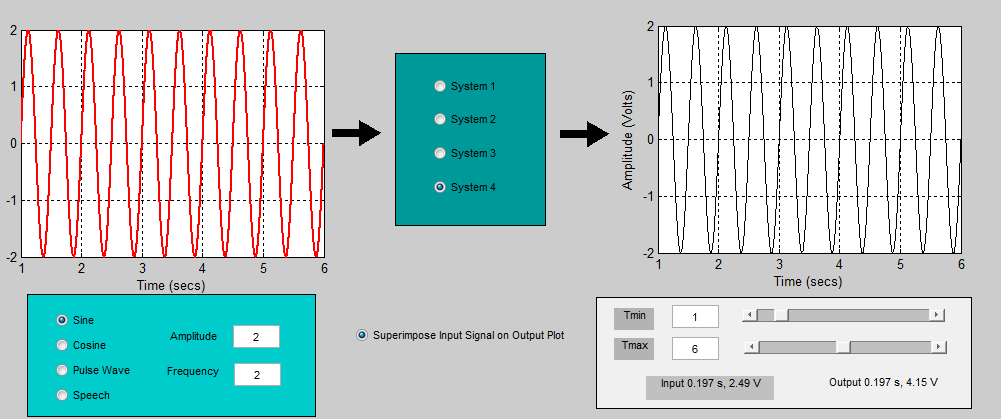
\includegraphics[height=1.75in]{S1P42.PNG}
\end{align*}\\

%\begin{figure}[H]
%	\centering
%	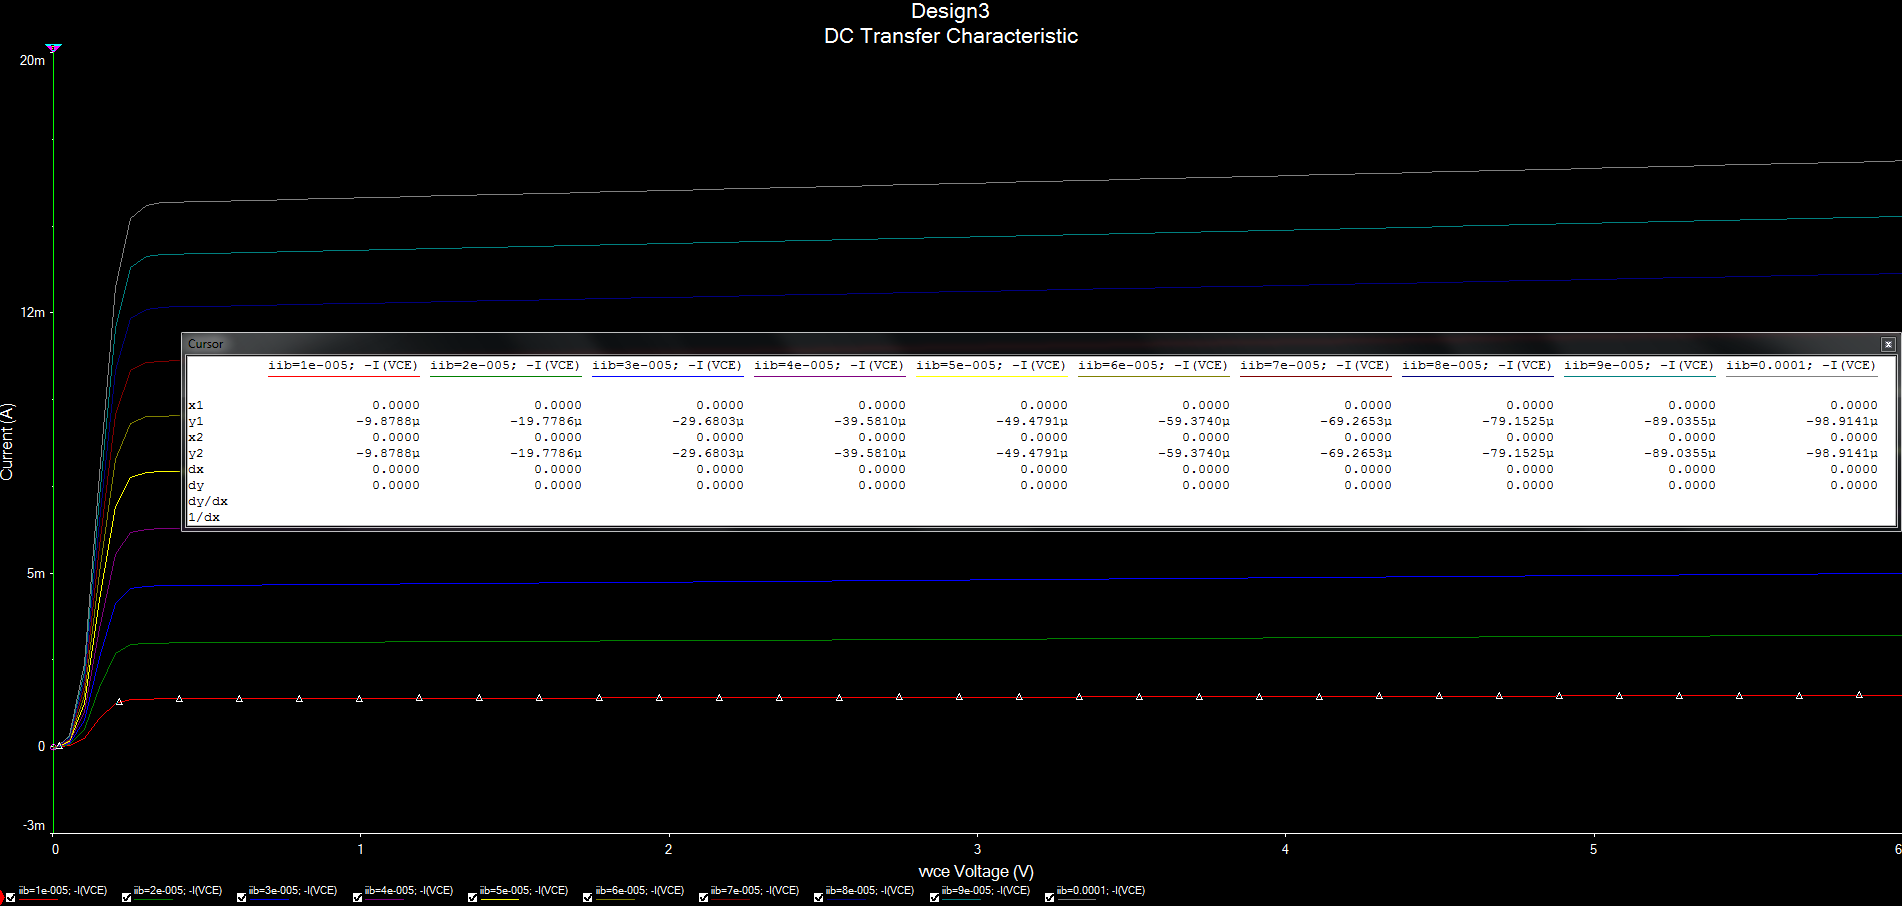
\includegraphics[height=3in]{/home/owner/Desktop/LAB REPORTS/D1/Pic7.PNG}
%	\caption[A.2 Part.7 Plot]{A.2 Part.7}
%	\label{fig:pic}
%\end{figure}


\pagebreak
\subsection{6.1 Gain and Phase as a function of frequency}

Q1. In your report complete the table below for the Sine input at various frequencies using system 1.\\
\\

\begin{table}[H]
\centering
\caption{6.1 Q1}
\label{tab:table 6.1}
\begin{tabular}{|c|c|c|c|l|l|l|l|}
\hline
\multicolumn{3}{|l|}{Input}                                                                                                                                                        & \multicolumn{5}{l|}{Output}                                                                                                                                                                                                                                                                                                                                                                \\ \hline
\begin{tabular}[c]{@{}c@{}}Frequency\\ (rad/sec)\end{tabular} & \begin{tabular}[c]{@{}c@{}}Frequency\\ (Hz)\end{tabular} & \begin{tabular}[c]{@{}c@{}}Amplitude\\ (x)\end{tabular} & \begin{tabular}[c]{@{}c@{}}Frequency\\ (rad/sec)\end{tabular} & \multicolumn{1}{c|}{\begin{tabular}[c]{@{}c@{}}Amplitude\\ (y)\end{tabular}} & \multicolumn{1}{c|}{\begin{tabular}[c]{@{}c@{}}Phase Lag\\ (sec)\end{tabular}} & \multicolumn{1}{c|}{\begin{tabular}[c]{@{}c@{}}Phase Lag\\ (rad)\end{tabular}} & \multicolumn{1}{c|}{\begin{tabular}[c]{@{}c@{}}Gain\\ (y/x)\end{tabular}} \\ \hline
1                                                             & 0.1591549                                                & 1                                                       & 1                                                             & 1.493                                                                        & 0.1011                                                                         & $ 4.9\times10^{-7} $                                                      & 1.493                                                                     \\ \hline
5                                                             & 0.7957745                                                & 1                                                       & 5                                                             & 1.342                                                                        & 0.092                                                                          & $ 4.66\times10^{-7}$                                                    & 1.342                                                                     \\ \hline
8                                                             & 1.2732392                                                & 1                                                       & 8                                                             & 1.171                                                                        & 0.085                                                                          & $ 4.12\times10^{-7}$                                                     & 1.171                                                                     \\ \hline
10                                                            & 1.591549                                                 & 1                                                       & 10                                                            & 1.212                                                                        & 0.085                                                                          & $ 4.12\times10^{-7}$                                                     & 1.212                                                                     \\ \hline
12                                                            & 1.9098588                                                & 1                                                       & 12                                                            & 0.9603                                                                       & 0.073                                                                          & $ 3.54\times10^{-7}$                                                     & 0.9603                                                                    \\ \hline
15                                                            & 2.3873235                                                & 1                                                       & 15                                                            & 0.832                                                                        & 0.066                                                                          & $ 3.2\times10^{-7}$                                                      & 0.832                                                                     \\ \hline
20                                                            & 3.183098                                                 & 1                                                       & 20                                                            & 0.6708                                                                       & 0.056                                                                          & $ 2.71\times10^{-7}$                                                     & 0.6708                                                                    \\ \hline
30                                                            & 4.774647                                                 & 1                                                       & 30                                                            & 0.4743                                                                       & 0.042                                                                          & $ 2.04\times10^{-7}$                                                     & 0.4743                                                                    \\ \hline
50                                                            & 7.952745                                                 & 1                                                       & 50                                                            & 0.2943                                                                       & 0.027                                                                          & $ 1.31\times10^{-7}$                                                     & 0.2943                                                                    \\ \hline
100                                                           & 15.91549                                                 & 1                                                       & 100                                                           & 0.1492                                                                       & 0.015                                                                          & $ 7.3\times10^{-8}$                                                      & 0.1492                                                                    \\ \hline
\end{tabular}
\end{table}

Q2. Plot a graph of Gain vs Frequency (rad/sec) and Phase (rad) vs Frequency (rad/sec) for system 1 using the information above. Label axes carefully.\\
\\

\begin{align*}
\centering
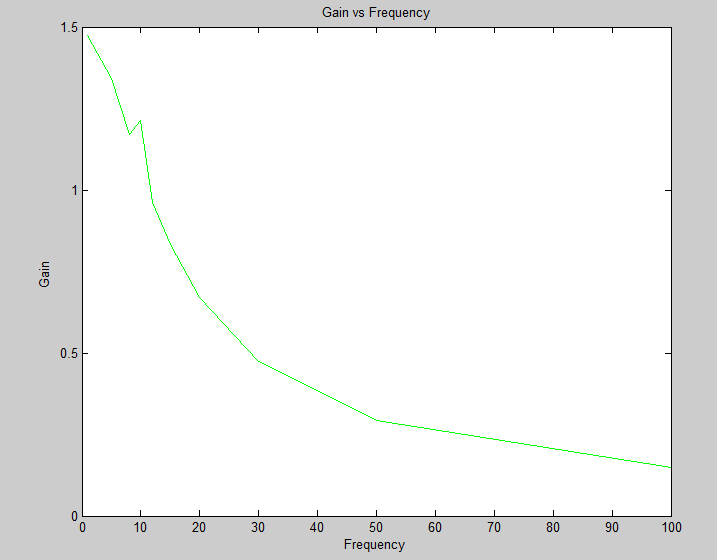
\includegraphics[height=1.75in]{S1P43.PNG}
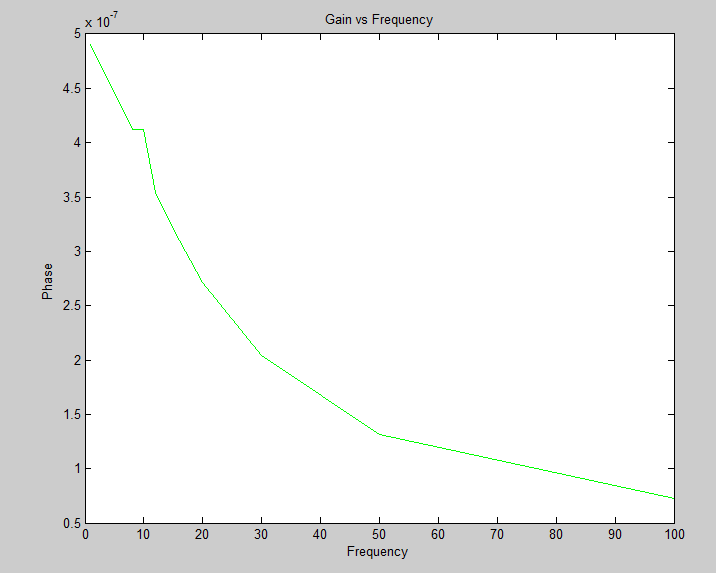
\includegraphics[height=1.75in]{S1P44.PNG}
\end{align*}


Q3. Is the effect of the system the same at all frequencies? How does the system behavior change with frequency?\\
\\

Ans3. The effect does change with frequency, it seems that the higher the input frequency becomes the lower the output Amplitude gets and the lower the phase lag also becomes. Due to the fact that the input Amplitude remained at a constant rate the Gain is easily determined and also found to be decreasing at the same rate as the Amplitude. \\

Q4. Discuss the significance of this plot with respect to the effect of system 1 on the Pulse Wave and the Speech Signal.
Ans4. The plot is very significant as it shows a near exponential decrease with respect to the increasing Frequency. Thus a systems gain can be easily manipulated by slightly changing the frequency to a lower or higher value.


\pagebreak


\section{Discussion}\label{sec:discuss}\underline{•}

The tools provided by the Matlab software are quite accurate thus the results were fairly accurate, the only limitation in them being the precision of the simulation software. The results obtained were also mostly theoretical as the actual signals would not be as ideal due to outside interference and environmental factors.\\

The values differed somewhat from the values obtained in the lectures as the simulation software provides some measure of realism , though not enough to be considered a true realistic value. The values obtained in the simulation would thus lie somewhere between the ideal and the real ones.
	\\
The advantages of having such a system is that complex functions can be simulated relatively quickly and assessed if they are the results wanted. The graphing and wave tools available also make discovering the right answer a very quick and trivial procedure.
Beyond those it also saves time and removes an aspect of the human error in calculating all the values by hand and then also having to graph them.
\\
The disadvantages of the simulation are of course the typical disadvantages in any simulation and that is that it is an approximation of a real value one would attain ignoring other environmental factors which might act on the system , such as temperature or time active.
\\
The huge advantages of simulation software is of course being far quick and more efficient with complex calculations which would take a human hours to do. 
It also allows for quick assessment and rectification to discover and repair mistakes.

	The disadvantages are the lack of variable the simulation usually has to take into account. Over engineering may be required in some parts to overcompensate for the lack of knowledge regarding certain aspects such as environment or temperature.\\


A methodical approach to building the design and calculating the functions used is always a good start. Progressive and accurate documentation of the results obtained and the procedure used to obtain those results is also neccesary. \\
The purpose of the experiment is to document the procedure and the results obtained so that the procedure can be reproduced accurately again.
\\



\pagebreak

\section{Conclusion}
LTI systems like all other signals have their limitations but that was not the point of this laboratory, The purpose of this laboratory was to show how easily a function can be mapped to a sine or cosine wave and then how easily that sine or cosine wave can be manipulated by increasing or decreasing the amplitude to give a distinctly different but similar wave. The overall purpose of this laboratory was to show the relationship between LTI systems and eigenvalues.
\\
	
	



\appendix
\section{References}
This is a list of links used for further information.

	\begin{enumerate}
	
	\item 3C1 Signals and Systems Notes
	\item Fundementals of Solid State Electronics, By Chih-Tang Sa
	\item Lab Description
	\end{enumerate}


\end{document}